\documentclass[10pt]{beamer}
%\usepackage[english]{babel}
\usepackage[utf8]{inputenc}
\usepackage[T1]{fontenc}
\usepackage{helvet}
\usepackage{listings}
%-------------------------------------------------------
% INFORMATION IN THE TITLE PAGE
%-------------------------------------------------------

\newcommand{\cstitle}{\textbf{Mineria de Datos}}
\subtitle[]{P4: Portable Parallel Processing Pipelines
	for Interactive Information Visualization}
\newcommand{\cscourseCode}{1704146}
\newcommand{\csauthor}{MSc. Vicente Machaca Arceda}
%\institute[UNSA]{Universidad Nacional de San Agustín de Arequipa}
\institute[UNSA]{\textbf{UNIVERSIDAD NACIONAL DE SAN AGUSTÍN}}
\newcommand{\csemail}{vmachacaa@unsa.edu.pe}
\newcommand{\instituteabr}{UNSA}
\newcommand{\nameUp}{ICC Fase 1}
\date{\today}
\title[\cscourseCode]{\cstitle}
\author{\csauthor}
%%%%%%%%%%%%%%%%%

%-------------------------------------------------------
% CHOOSE THE THEME
%-------------------------------------------------------
\def\mycmd{0} % CS THEME
\def\mycmd{1} % MYTHEME
%-------------------------------------------------------

\newcommand{\namelogo}{img/2.png}

\if\mycmd1
\usetheme[]{Feather}
\newcommand{\chref}[2]{	\href{#1}{{\usebeamercolor[bg]{Feather}#2}} }
\else
\usepackage{csformat}
\fi

\newcommand{\1}{
	\setbeamertemplate{background}{
		
\includegraphics[width=\paperwidth,height=\paperheight]{img/1}
		\tikz[overlay] \fill[fill opacity=0.75,fill=white] (0,0) rectangle (-\paperwidth,\paperheight);
	}
}


\usepackage[spanish]{babel}
\AtBeginDocument{\selectlanguage{spanish}}
\renewcommand{\figurename}{Figura}
\renewcommand{\refname}{Referencias}
\renewcommand{\tablename}{Tabla}



%-------------------------------------------------------
% THE BODY OF THE PRESENTATION
%-------------------------------------------------------

\begin{document}
	
	
\AtBeginSubsection[]
{
\begin{frame}
\frametitle{Tabla de contenido}
\tableofcontents[currentsubsection]
\end{frame}
}


%-------------------------------------------------------
% THE TITLEPAGE
%-------------------------------------------------------

\if\mycmd1 % MY THEME
\1{
\begin{frame}[plain,noframenumbering] 
\titlepage 
\end{frame}}

\else % CS THEME
\maketitle
\fi


%-------------------------------------------------------
%-------------------------------------------------------
\begin{frame}{Tabla de contenido}
\tableofcontents
\end{frame}
%-------------------------------------------------------
%-------------------------------------------------------




%%%%%%%%%%%%%%%%%%%%%%%%%%%%%%%%%%%%%%%%%%%%%%%%%%%%%%%%%%%%%%%%%%%%%%%%%%%%%%%%%%%%%%%%%%%%%%%%%%%%%%%%%%%%%%%%
%%%%%%%%%%%%%%%%%%%%%%%%%%%%%%%%%%%%%%%%%%%%%%%%%%%%%%%%%%%%%%%%%%%%%%%%%%%%%%%%%%%%%%%%%%%%%%%%%%%%%%%%%%%%%%%%
\section{Introducción}
%%%%%%%%%%%%%%%%%%%%%%%%%%%%%%%%%%%%%%%%%%%%%%%%%%%%%%%%%%%%%%%%%%%%%%%%%%%%%%%%%%%%%%%%%%%%%%%%%%%%%%%%%%%%%%%%
%%%%%%%%%%%%%%%%%%%%%%%%%%%%%%%%%%%%%%%%%%%%%%%%%%%%%%%%%%%%%%%%%%%%%%%%%%%%%%%%%%%%%%%%%%%%%%%%%%%%%%%%%%%%%%%%

%-------------------------------------------------------
%-------------------------------------------------------
\begin{frame}{Introducción}{Visualización de datos}
\begin{columns}
	\begin{column}{0.48\textwidth}
		\begin{figure}[]
			\centering
			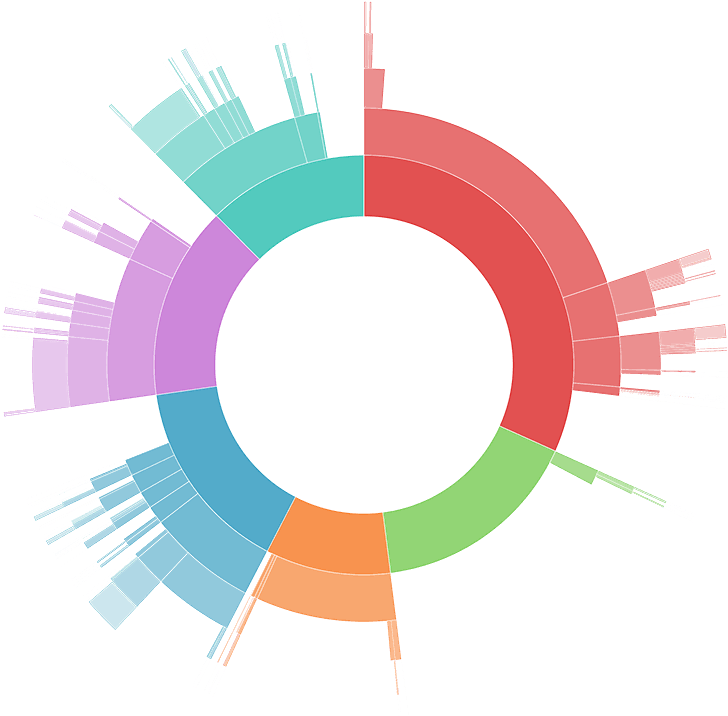
\includegraphics[width=\textwidth,height=0.5\textheight,keepaspectratio]{img/mineria/p4_2}
			%\label{img:mot2}
			\caption{Ejemplo de visualización de datos.}
		\end{figure}	
	\end{column}
	\begin{column}{0.48\textwidth}
		La visualización de datos a probado ser efectiva para el razonamiento de grandes volumenes de datos			\cite{card1999readings}.			
	\end{column}
\end{columns}
\end{frame}
%-------------------------------------------------------
%-------------------------------------------------------


%-------------------------------------------------------
%-------------------------------------------------------
\begin{frame}{Introducción}{Gramáticas declarativas para visualización de datos}

\begin{itemize}
	\item\textbf{D$^3$} data-driven documents \cite{bostock2011d3}.
	\item \textbf{ggplot2}: elegant graphics for data analysis \cite{wickham2016ggplot2}.
	\item \textbf{Reactive vega}: A streaming dataflow architecture for declarative interactive visualization \cite{satyanarayan2015reactive}.
	\item \textbf{Vega-lite}: A grammar of interactive graphics \cite{satyanarayan2016vega}.
	
\end{itemize}

\end{frame}
%-------------------------------------------------------
%-------------------------------------------------------

%-------------------------------------------------------
%-------------------------------------------------------
\begin{frame}{Introducción}{Gramáticas declarativas para visualización de datos}
\begin{columns}
	\begin{column}{0.48\textwidth}
		\begin{figure}[]
			\centering
			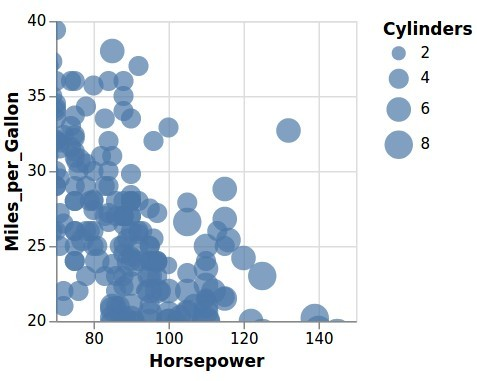
\includegraphics[width=\textwidth,height=0.4\textheight,keepaspectratio]{img/mineria/p4_3}
			%\label{img:mot2}
			\caption{Scatterplot en Vega-lite.}
		\end{figure}	
	\end{column}
	\begin{column}{0.48\textwidth}
		\begin{figure}[]
			\centering
			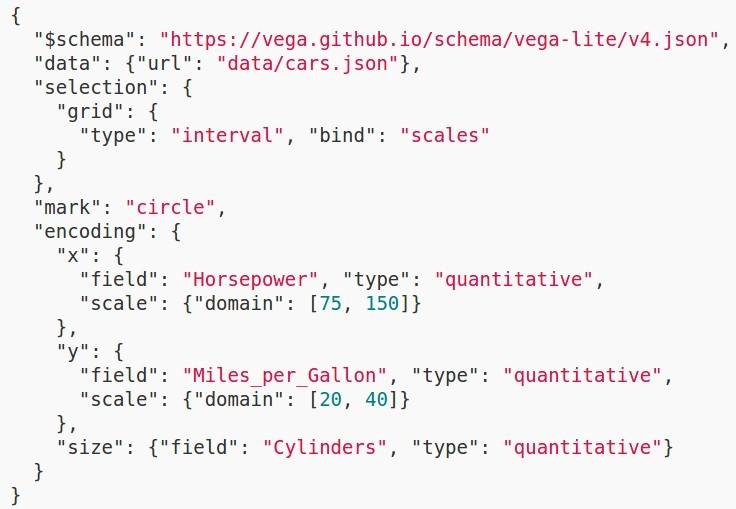
\includegraphics[width=\textwidth,height=0.7\textheight,keepaspectratio]{img/mineria/p4_4}
			%\label{img:mot2}
			%\caption{Scatterplot en Vega-lite.}
		\end{figure}	
	\end{column}
\end{columns}
\end{frame}
%-------------------------------------------------------
%-------------------------------------------------------


%-------------------------------------------------------
%-------------------------------------------------------
\begin{frame}{Introducción}{Problema}	
\begin{block}{Problema}
	La mayoría de software de visualización de datos, no hacen uso del procesamiento paralelo para construir sistemas interactivos de alto desempeño \cite{li2018p4}.		
\end{block}
\pause
\begin{block}{Propuesta}
	El paper presenta \textbf{P4}, un software de vizualización. P4 hace uso de un lenguaje declarativo y aprovecha el poder computacional del GPU.		
\end{block}	
\end{frame}
%-------------------------------------------------------
%-------------------------------------------------------

%%%%%%%%%%%%%%%%%%%%%%%%%%%%%%%%%%%%%%%%%%%%%%%%%%%%%%%%%%%%%%%%%%%%%%%%%%%%%%%%%%%%%%%%%%%%%%%%%%%%%%%%%%%%%%%%
%%%%%%%%%%%%%%%%%%%%%%%%%%%%%%%%%%%%%%%%%%%%%%%%%%%%%%%%%%%%%%%%%%%%%%%%%%%%%%%%%%%%%%%%%%%%%%%%%%%%%%%%%%%%%%%%
%\section{Estado del arte}
%%%%%%%%%%%%%%%%%%%%%%%%%%%%%%%%%%%%%%%%%%%%%%%%%%%%%%%%%%%%%%%%%%%%%%%%%%%%%%%%%%%%%%%%%%%%%%%%%%%%%%%%%%%%%%%%
%%%%%%%%%%%%%%%%%%%%%%%%%%%%%%%%%%%%%%%%%%%%%%%%%%%%%%%%%%%%%%%%%%%%%%%%%%%%%%%%%%%%%%%%%%%%%%%%%%%%%%%%%%%%%%%%

%-------------------------------------------------------
%-------------------------------------------------------
%\begin{frame}{Estado del arte}{Herramientas gráficas de visualización}	
%\begin{itemize}
%	\item Existen muchas herramientas para la visualización de datos con gramáticas declarativas. \pause
%	\item Dichas herramientas utilizan solo el CPU. \pause
%	\item La adopción del GPU es lenta debido a su complejidad. \pause
%	\item Algunos enfoques se basan en la adopción de OpenGL, WebGL y CUDA.
%\end{itemize}
%\end{frame}
%-------------------------------------------------------
%-------------------------------------------------------


%-------------------------------------------------------
%-------------------------------------------------------
%\begin{frame}{Estado del arte}{Técnicas de visualización de alto desempeño}	
%\begin{itemize}
%	\item Métodos de reducción han sido aplicados: filtering, sampling y data cubes. \pause
%	\item Tambien se ha aplicado mulithreading en CPUs. \pause
%	\item Otros métodos toman ventaja del uso del GPU. \pause
%\end{itemize}
%\end{frame}
%-------------------------------------------------------
%-------------------------------------------------------


%%%%%%%%%%%%%%%%%%%%%%%%%%%%%%%%%%%%%%%%%%%%%%%%%%%%%%%%%%%%%%%%%%%%%%%%%%%%%%%%%%%%%%%%%%%%%%%%%%%%%%%%%%%%%%%%
%%%%%%%%%%%%%%%%%%%%%%%%%%%%%%%%%%%%%%%%%%%%%%%%%%%%%%%%%%%%%%%%%%%%%%%%%%%%%%%%%%%%%%%%%%%%%%%%%%%%%%%%%%%%%%%%
\section{P4}
%%%%%%%%%%%%%%%%%%%%%%%%%%%%%%%%%%%%%%%%%%%%%%%%%%%%%%%%%%%%%%%%%%%%%%%%%%%%%%%%%%%%%%%%%%%%%%%%%%%%%%%%%%%%%%%%
%%%%%%%%%%%%%%%%%%%%%%%%%%%%%%%%%%%%%%%%%%%%%%%%%%%%%%%%%%%%%%%%%%%%%%%%%%%%%%%%%%%%%%%%%%%%%%%%%%%%%%%%%%%%%%%%

%%%%%%%%%%%%%%%%%%%%%%%%%%%%%%%%%%%%%%%%%%%%%%%%%%%%%%%%%%%%%%%%%%%%%%%%%%%%%%%%%%%%%%%%%%%%%%%%%%%%%%%%%%%%%%%%
%%%%%%%%%%%%%%%%%%%%%%%%%%%%%%%%%%%%%%%%%%%%%%%%%%%%%%%%%%%%%%%%%%%%%%%%%%%%%%%%%%%%%%%%%%%%%%%%%%%%%%%%%%%%%%%%
\subsection{Arquitectura}
%%%%%%%%%%%%%%%%%%%%%%%%%%%%%%%%%%%%%%%%%%%%%%%%%%%%%%%%%%%%%%%%%%%%%%%%%%%%%%%%%%%%%%%%%%%%%%%%%%%%%%%%%%%%%%%%
%%%%%%%%%%%%%%%%%%%%%%%%%%%%%%%%%%%%%%%%%%%%%%%%%%%%%%%%%%%%%%%%%%%%%%%%%%%%%%%%%%%%%%%%%%%%%%%%%%%%%%%%%%%%%%%%


%-------------------------------------------------------
%-------------------------------------------------------
\begin{frame}{Arquitectura de P4}
\begin{figure}[]
	\centering
	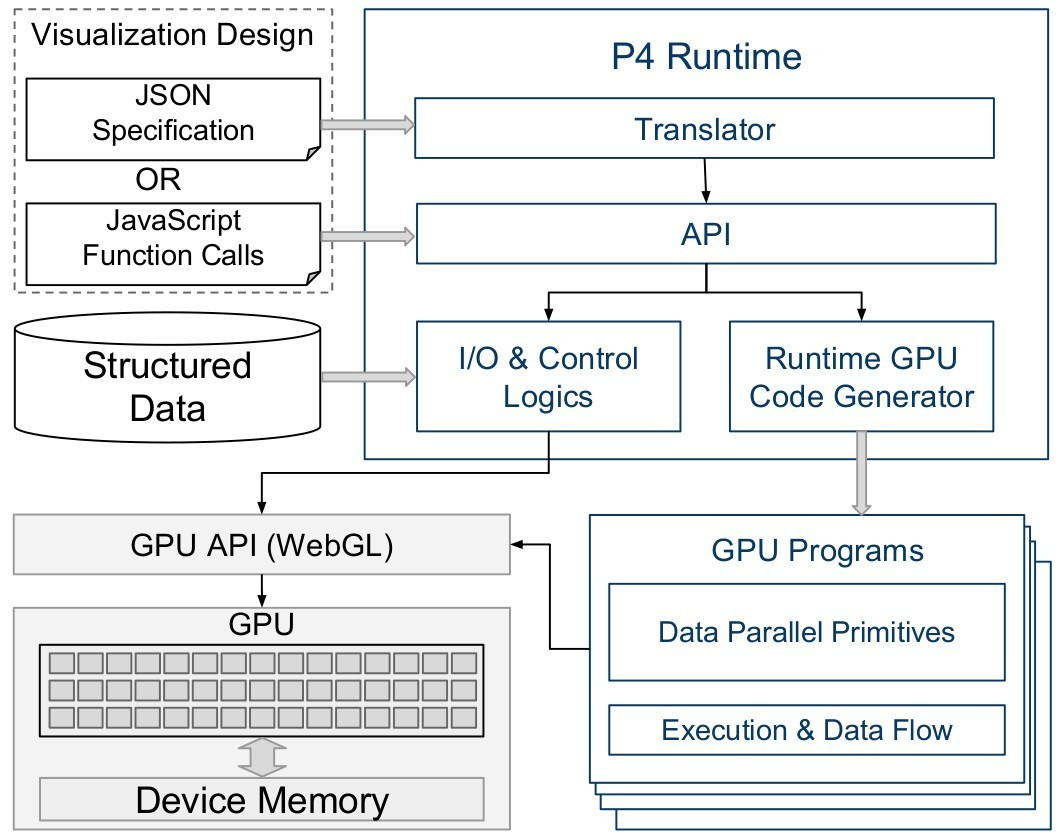
\includegraphics[width=0.7\textwidth,keepaspectratio]{img/mineria/p4_5}
	%\label{img:mot2}
	\caption{Arquitectura de P4. Fuente: \cite{li2018p4}}
\end{figure}	
\end{frame}
%-------------------------------------------------------
%-------------------------------------------------------

%%%%%%%%%%%%%%%%%%%%%%%%%%%%%%%%%%%%%%%%%%%%%%%%%%%%%%%%%%%%%%%%%%%%%%%%%%%%%%%%%%%%%%%%%%%%%%%%%%%%%%%%%%%%%%%%
%%%%%%%%%%%%%%%%%%%%%%%%%%%%%%%%%%%%%%%%%%%%%%%%%%%%%%%%%%%%%%%%%%%%%%%%%%%%%%%%%%%%%%%%%%%%%%%%%%%%%%%%%%%%%%%%
\subsection{Interfaces de programación}
%%%%%%%%%%%%%%%%%%%%%%%%%%%%%%%%%%%%%%%%%%%%%%%%%%%%%%%%%%%%%%%%%%%%%%%%%%%%%%%%%%%%%%%%%%%%%%%%%%%%%%%%%%%%%%%%
%%%%%%%%%%%%%%%%%%%%%%%%%%%%%%%%%%%%%%%%%%%%%%%%%%%%%%%%%%%%%%%%%%%%%%%%%%%%%%%%%%%%%%%%%%%%%%%%%%%%%%%%%%%%%%%%

%-------------------------------------------------------
%-------------------------------------------------------
\begin{frame}{Interfaces de programación de P4}{Base de datos de los ejemplos}
\begin{block}{}
	Se utilizará una base de datos de nacimientos del 2015 (200000 muestras). Los atributos son:
	
	\begin{columns}
		\begin{column}{0.48\textwidth}
			\begin{itemize}
				\item Mes de nacimiento.
				\item Genero del bebe.
				\item Peso del bebe.
				\item Edad de la madre.
				\item Raza de la madre.
				\item Estado civil de la madre.
				\item Grado de educación de la madre.
			\end{itemize}
		\end{column}
		\begin{column}{0.48\textwidth}
			\begin{itemize}
				\item Altura de la madre.
				\item Peso de la madre.
				\item Aumento de peso de la madre durante el embarazo.
				\item Edad del padre
				\item Raza del padre.
				\item Grado de educación del padre.
			\end{itemize}	
		\end{column}
	\end{columns}
	
	
\end{block}
\end{frame}
%-------------------------------------------------------
%-------------------------------------------------------


%-------------------------------------------------------
%-------------------------------------------------------
\begin{frame}{Interfaces de programación de P4}{Transformación de datos}
\begin{block}{Transformación de datos}
	\begin{itemize}
		\item \textbf{Derive}.- Genera nuevos atributos. 
		\item \textbf{Match}.- Filtra los  atributos.
		\item \textbf{Aggregate}.- Agrupa atributos. 
	\end{itemize}
\end{block}	
\end{frame}
%-------------------------------------------------------
%-------------------------------------------------------

%-------------------------------------------------------
%-------------------------------------------------------
\begin{frame}{Interfaces de programación de P4}{Transformación de datos}
\begin{figure}[]
	\centering
	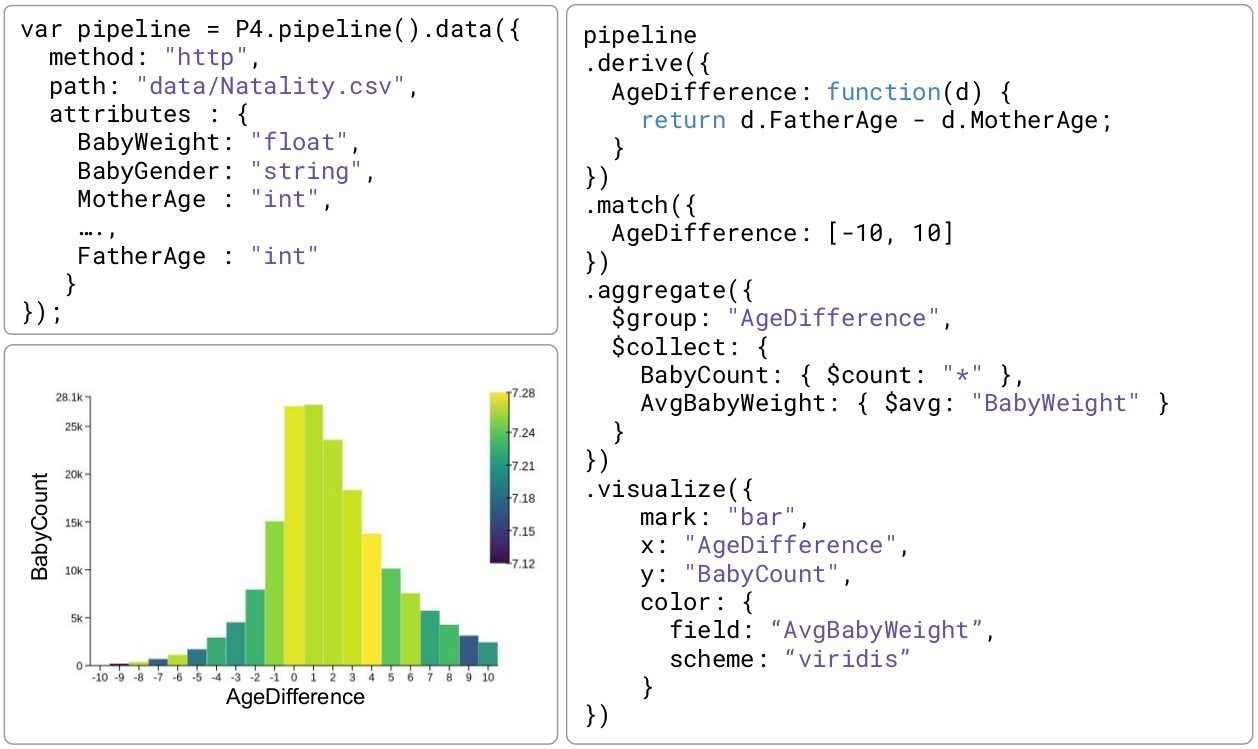
\includegraphics[width=0.95\textwidth,keepaspectratio]{img/mineria/p4_6}
	%\label{img:mot2}
	\caption{Ejemplo de transformación de datos con P4. Fuente: \cite{li2018p4}}
\end{figure}
\end{frame}
%-------------------------------------------------------
%-------------------------------------------------------

%-------------------------------------------------------
%-------------------------------------------------------
\begin{frame}{Interfaces de programación de P4}{Mapeo visual}
\begin{block}{Mapeo visual}
	Permite que los atributos se renderizen de manera facil a canales visuales como: color, opacidad, ancho, altura, posición del eje \textit{x} y eje \textit{y}.
\end{block}	
\end{frame}
%-------------------------------------------------------
%-------------------------------------------------------

%-------------------------------------------------------
%-------------------------------------------------------
\begin{frame}{Interfaces de programación de P4}{Mapeo visual}
\begin{figure}[]
	\centering
	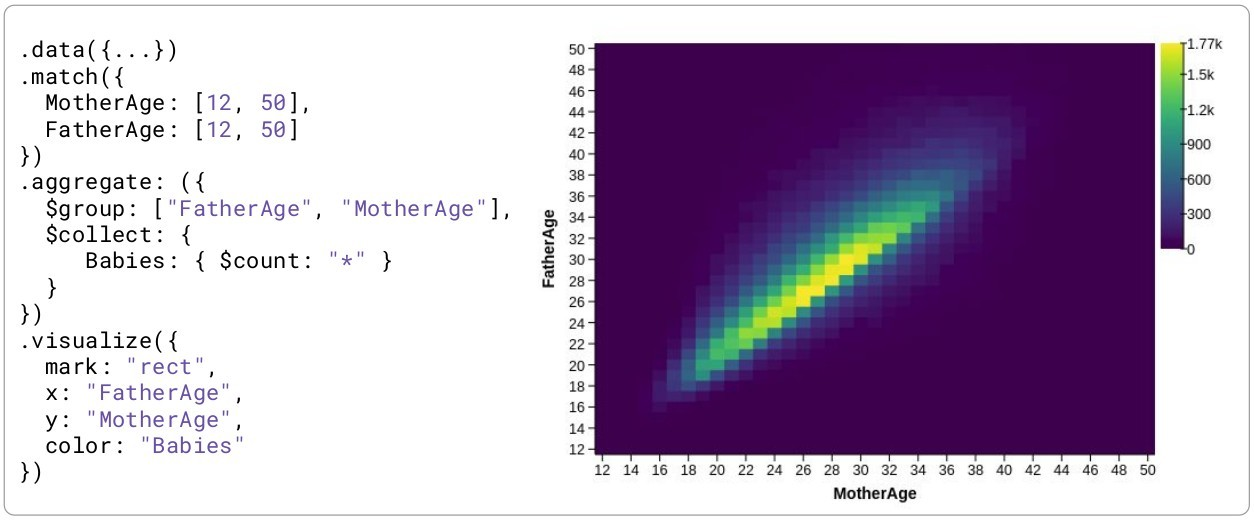
\includegraphics[width=\textwidth,keepaspectratio]{img/mineria/p4_8}
	%\label{img:mot2}
	\caption{Ejemplo de visualización de datos con P4. Fuente: \cite{li2018p4}}
\end{figure}
\end{frame}
%-------------------------------------------------------
%-------------------------------------------------------

%-------------------------------------------------------
%-------------------------------------------------------
\begin{frame}{Interfaces de programación de P4}{Mapeo visual}
\begin{figure}[]
	\centering
	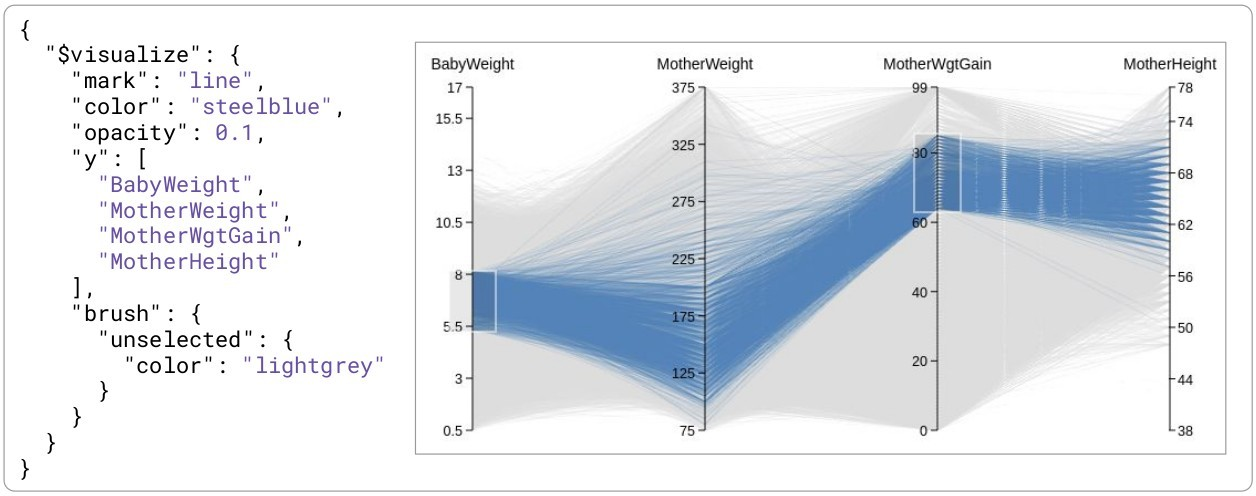
\includegraphics[width=\textwidth,keepaspectratio]{img/mineria/p4_9}
	%\label{img:mot2}
	\caption{Ejemplo de visualización de datos con P4. Fuente: \cite{li2018p4}}
\end{figure}
\end{frame}
%-------------------------------------------------------
%-------------------------------------------------------


%-------------------------------------------------------
%-------------------------------------------------------
\begin{frame}{Interfaces de programación de P4}{Interacciones}
\begin{figure}[]
	\centering
	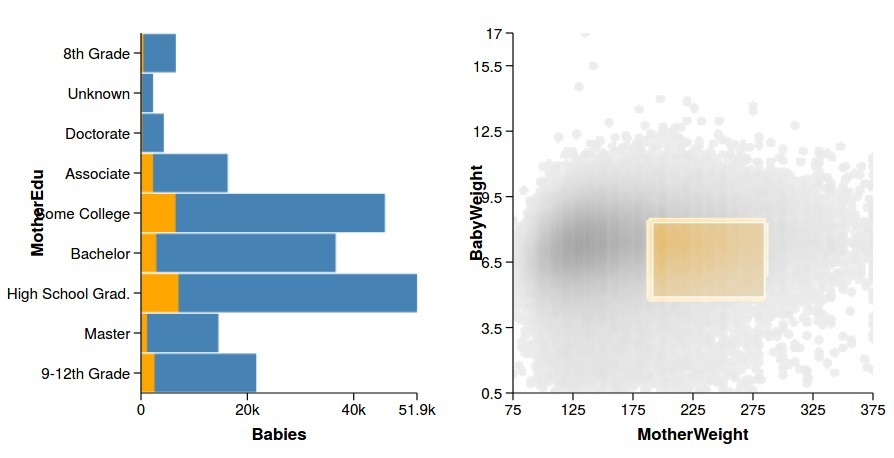
\includegraphics[width=\textwidth,keepaspectratio]{img/mineria/p4_10}
	%\label{img:mot2}
	\caption{Ejemplo de interacciones con P4. Fuente: \cite{li2018p4}}
\end{figure}
\end{frame}
%-------------------------------------------------------
%-------------------------------------------------------



%-------------------------------------------------------
%-------------------------------------------------------
\begin{frame}{Interfaces de programación de P4}{Mejora de percepción}
\begin{block}{}
	P4, mejora la reducción del ruido al mostrar grandes volumenes de datos. Esto lo logra procesando la opacidad en cada pixel $\hat{\alpha}$ con:
	
	\[
	\hat{\alpha} = (1 - \alpha_{min})( \frac{p}{p_{max}} )^\gamma + \alpha_{min}
	\]
	Donde: \\
	\begin{itemize}
		\item $p$: Número de marcas sobrepuestas en pixel actual.
		\item $p_{max}$: Máximo número de marcas sobrepuestas en toda la imagen.
		\item $\gamma = 1/3$
		\item $\alpha_{min} = 0.1$
		
	\end{itemize}
	
\end{block}
\end{frame}
%-------------------------------------------------------
%-------------------------------------------------------


%-------------------------------------------------------
%-------------------------------------------------------
\begin{frame}{Interfaces de programación de P4}{Mejora de percepción}
\begin{figure}[]
	\centering
	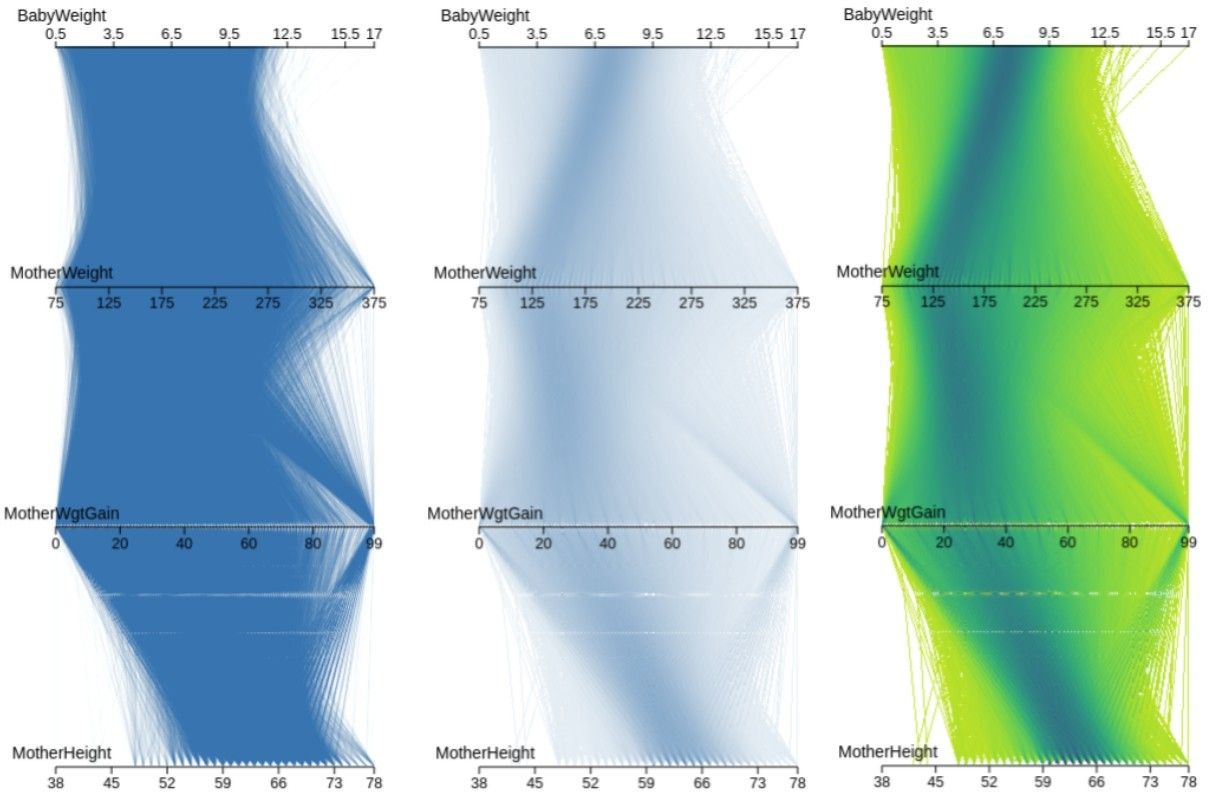
\includegraphics[width=0.8\textwidth,keepaspectratio]{img/mineria/p4_11}
	%\label{img:mot2}
	\caption{Izquierda: Alpha blending de WebGL, Centro: Ajuste de opacidad con P4, Derecha: Mapeo de color con P4. Fuente: \cite{li2018p4}}
\end{figure}
\end{frame}
%-------------------------------------------------------
%-------------------------------------------------------




%%%%%%%%%%%%%%%%%%%%%%%%%%%%%%%%%%%%%%%%%%%%%%%%%%%%%%%%%%%%%%%%%%%%%%%%%%%%%%%%%%%%%%%%%%%%%%%%%%%%%%%%%%%%%%%%
%%%%%%%%%%%%%%%%%%%%%%%%%%%%%%%%%%%%%%%%%%%%%%%%%%%%%%%%%%%%%%%%%%%%%%%%%%%%%%%%%%%%%%%%%%%%%%%%%%%%%%%%%%%%%%%%
\subsection{Framework de procesamiento paralelo}
%%%%%%%%%%%%%%%%%%%%%%%%%%%%%%%%%%%%%%%%%%%%%%%%%%%%%%%%%%%%%%%%%%%%%%%%%%%%%%%%%%%%%%%%%%%%%%%%%%%%%%%%%%%%%%%%
%%%%%%%%%%%%%%%%%%%%%%%%%%%%%%%%%%%%%%%%%%%%%%%%%%%%%%%%%%%%%%%%%%%%%%%%%%%%%%%%%%%%%%%%%%%%%%%%%%%%%%%%%%%%%%%%



%-------------------------------------------------------
%-------------------------------------------------------
\begin{frame}{Framework de procesamiento paralelo}{Primitivas}
\begin{block}{Primitivas de paralelización}
	Las operaciones de P4, pueden ser implementadas como las primitivas de programación funcional: \textit{map}, \textit{filter} y \textit{reduce}. Entonces, si se implemnta dichas primitivas funcionales en GPU, se soluciona el problema de paralelización de P4. 
	
	\vspace{0.3cm}
	
	P4 tiene cuatro primitivas:
	
	\begin{itemize}
		\item Fetch.
		\item Map.
		\item Filter.
		\item Reduce.
	\end{itemize}
	
\end{block}
\end{frame}
%-------------------------------------------------------
%-------------------------------------------------------

%-------------------------------------------------------
%-------------------------------------------------------
\begin{frame}{Framework de procesamiento paralelo}{\textit{map}, \textit{filter} y \textit{reduce}}
\begin{figure}[]
	\centering
	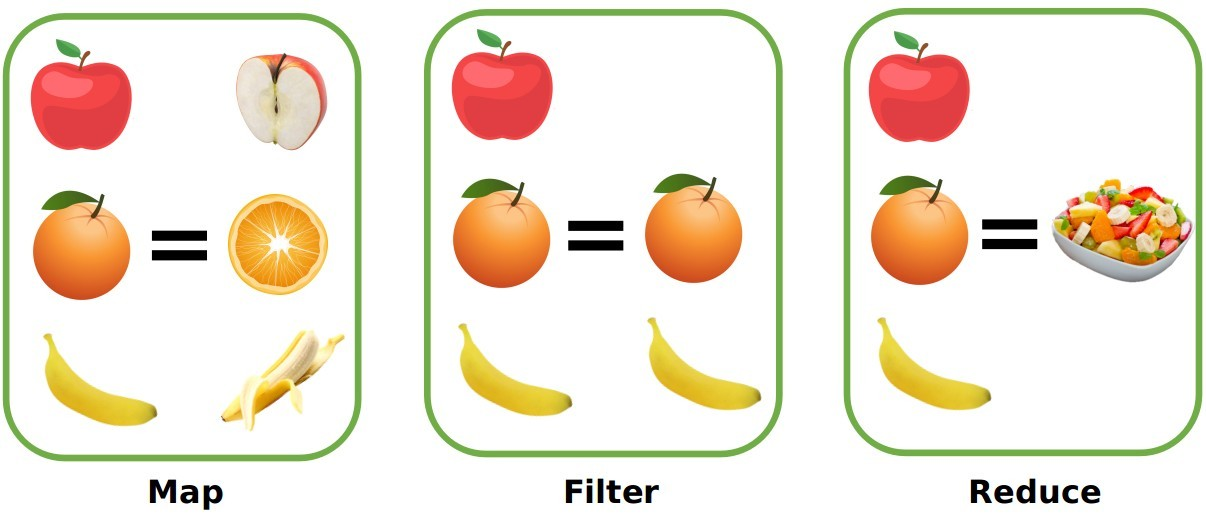
\includegraphics[width=\textwidth,keepaspectratio]{img/mineria/map_filter_reduce.jpg}
	%\label{img:mot2}
	\caption{Ejemplo de \textit{map}, \textit{filter} y \textit{reduce} utilizados en programación funcional.}
\end{figure}
\end{frame}
%-------------------------------------------------------
%-------------------------------------------------------


%-------------------------------------------------------
%-------------------------------------------------------
\begin{frame}{Framework de procesamiento paralelo}{Primitivas}
\begin{figure}[]
	\centering
	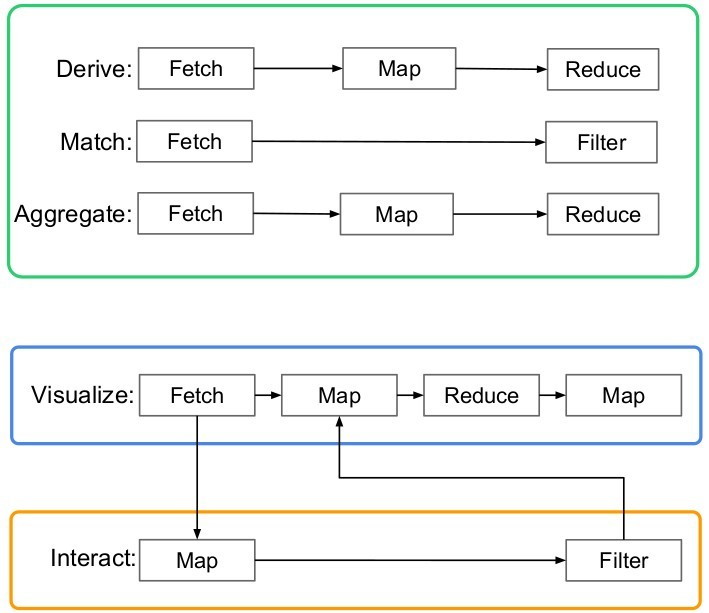
\includegraphics[width=0.6\textwidth,keepaspectratio]{img/mineria/p4_12}
	%\label{img:mot2}
	\caption{Framework para el procesamiento paralelo de P4. Fuente: \cite{li2018p4}}
\end{figure}
\end{frame}
%-------------------------------------------------------
%-------------------------------------------------------


%-------------------------------------------------------
%-------------------------------------------------------
\begin{frame}{Framework de procesamiento paralelo}{\textit{Vertex shader} y \textit{Fragment shader}}
\begin{figure}[]
	\centering
	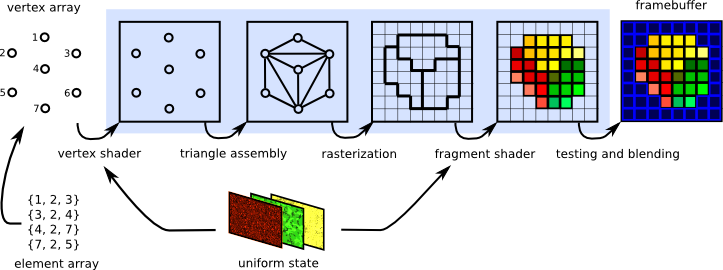
\includegraphics[width=\textwidth,keepaspectratio]{img/mineria/webgl.png}
	%\label{img:mot2}
	\caption{Ejemplo de \textit{Vertex shader} y \textit{Fragment shader} en WebGL.}
\end{figure}
\end{frame}
%-------------------------------------------------------
%-------------------------------------------------------

%-------------------------------------------------------
%-------------------------------------------------------
\begin{frame}{Framework de procesamiento paralelo}{Primitivas}
\begin{itemize}
    \item \textbf{Fetch}.- La información se almacena como texturas y se usan los shader para acceder a la información.\pause
    \item \textbf{Map}.- \textit{Vertex shader} para procesar resultados intermedios. \textit{Fragment shader} para escribir los resultados.\pause
    \item \textbf{Filter}.- \textit{Vertex shader} para el filtro. \textit{Fragment shader} para guardar los resultados.\pause
     \item \textbf{Reduce}.- Uiliza  \textit{blending} para obtener los máximos, mínimos, etc.
\end{itemize}

\end{frame}
%-------------------------------------------------------
%-------------------------------------------------------

%%%%%%%%%%%%%%%%%%%%%%%%%%%%%%%%%%%%%%%%%%%%%%%%%%%%%%%%%%%%%%%%%%%%%%%%%%%%%%%%%%%%%%%%%%%%%%%%%%%%%%%%%%%%%%%%
%%%%%%%%%%%%%%%%%%%%%%%%%%%%%%%%%%%%%%%%%%%%%%%%%%%%%%%%%%%%%%%%%%%%%%%%%%%%%%%%%%%%%%%%%%%%%%%%%%%%%%%%%%%%%%%%
\section{Resultados}
%%%%%%%%%%%%%%%%%%%%%%%%%%%%%%%%%%%%%%%%%%%%%%%%%%%%%%%%%%%%%%%%%%%%%%%%%%%%%%%%%%%%%%%%%%%%%%%%%%%%%%%%%%%%%%%%
%%%%%%%%%%%%%%%%%%%%%%%%%%%%%%%%%%%%%%%%%%%%%%%%%%%%%%%%%%%%%%%%%%%%%%%%%%%%%%%%%%%%%%%%%%%%%%%%%%%%%%%%%%%%%%%%


%-------------------------------------------------------
%-------------------------------------------------------
\begin{frame}{Benchmark}{Librerías}
\begin{table}[]
	\caption{Librerías utilizadas para la comparación con P4.}
	\begin{tabular}{ll}
		\hline
		Libreria  & Versión \\ \hline
		$D^3$        & 3.5.17  \\
		Vega      & 3.0.2   \\
		Lodash    & 4.17.4  \\
		Startdust & 0.1.1  
	\end{tabular}
\end{table}
\end{frame}
%-------------------------------------------------------
%-------------------------------------------------------

%-------------------------------------------------------
%-------------------------------------------------------
\begin{frame}{Benchmark}{GPUs utilizadas}
\begin{table}[]
	\caption{Tarjetas GPU utilizadas en los experimentos.}
	\begin{tabular}{llll}
		\hline
		Fabricante  & Modelo & Nucleos & Memoria \\ \hline
		Intel &  HD520 & 192 & 1GB DDR3 \\
		Nvidia  &  GTX940m & 384 & 2GB DDR3 \\
		AMD  &  HD7970 & 2048 & 3GB DDR5 \\
		Nvidia &  GTXTitan & 2688 & 6GB DDR5 \\
	\end{tabular}
\end{table}
\end{frame}
%-------------------------------------------------------
%-------------------------------------------------------

%-------------------------------------------------------
%-------------------------------------------------------
\begin{frame}{Benchmark}{Desempeño en la transformación de datos}
	\begin{figure}[]
		\centering
		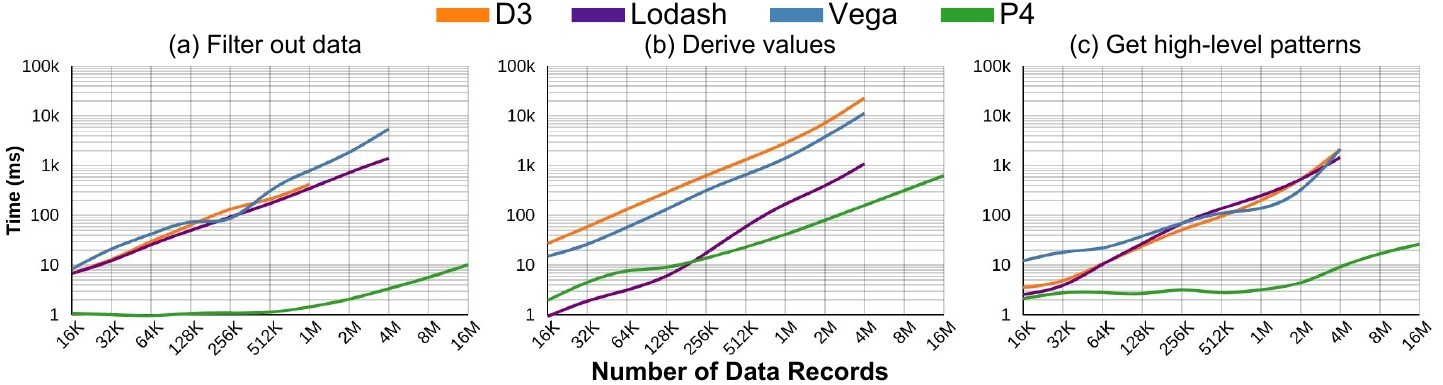
\includegraphics[width=\textwidth,keepaspectratio]{img/mineria/p4_13}
		%\label{img:mot2}
		\caption{Tiempo promedio de P4 y las demas librerías para procesar las tareas de \textit{Match}, \textit{Derive} y \textit{Aggregate}. Fuente: \cite{li2018p4}}
	\end{figure}
\end{frame}
%-------------------------------------------------------
%-------------------------------------------------------

%-------------------------------------------------------
%-------------------------------------------------------
\begin{frame}{Benchmark}{Desempeño en la transformación de datos}
	\begin{figure}[]
		\centering
		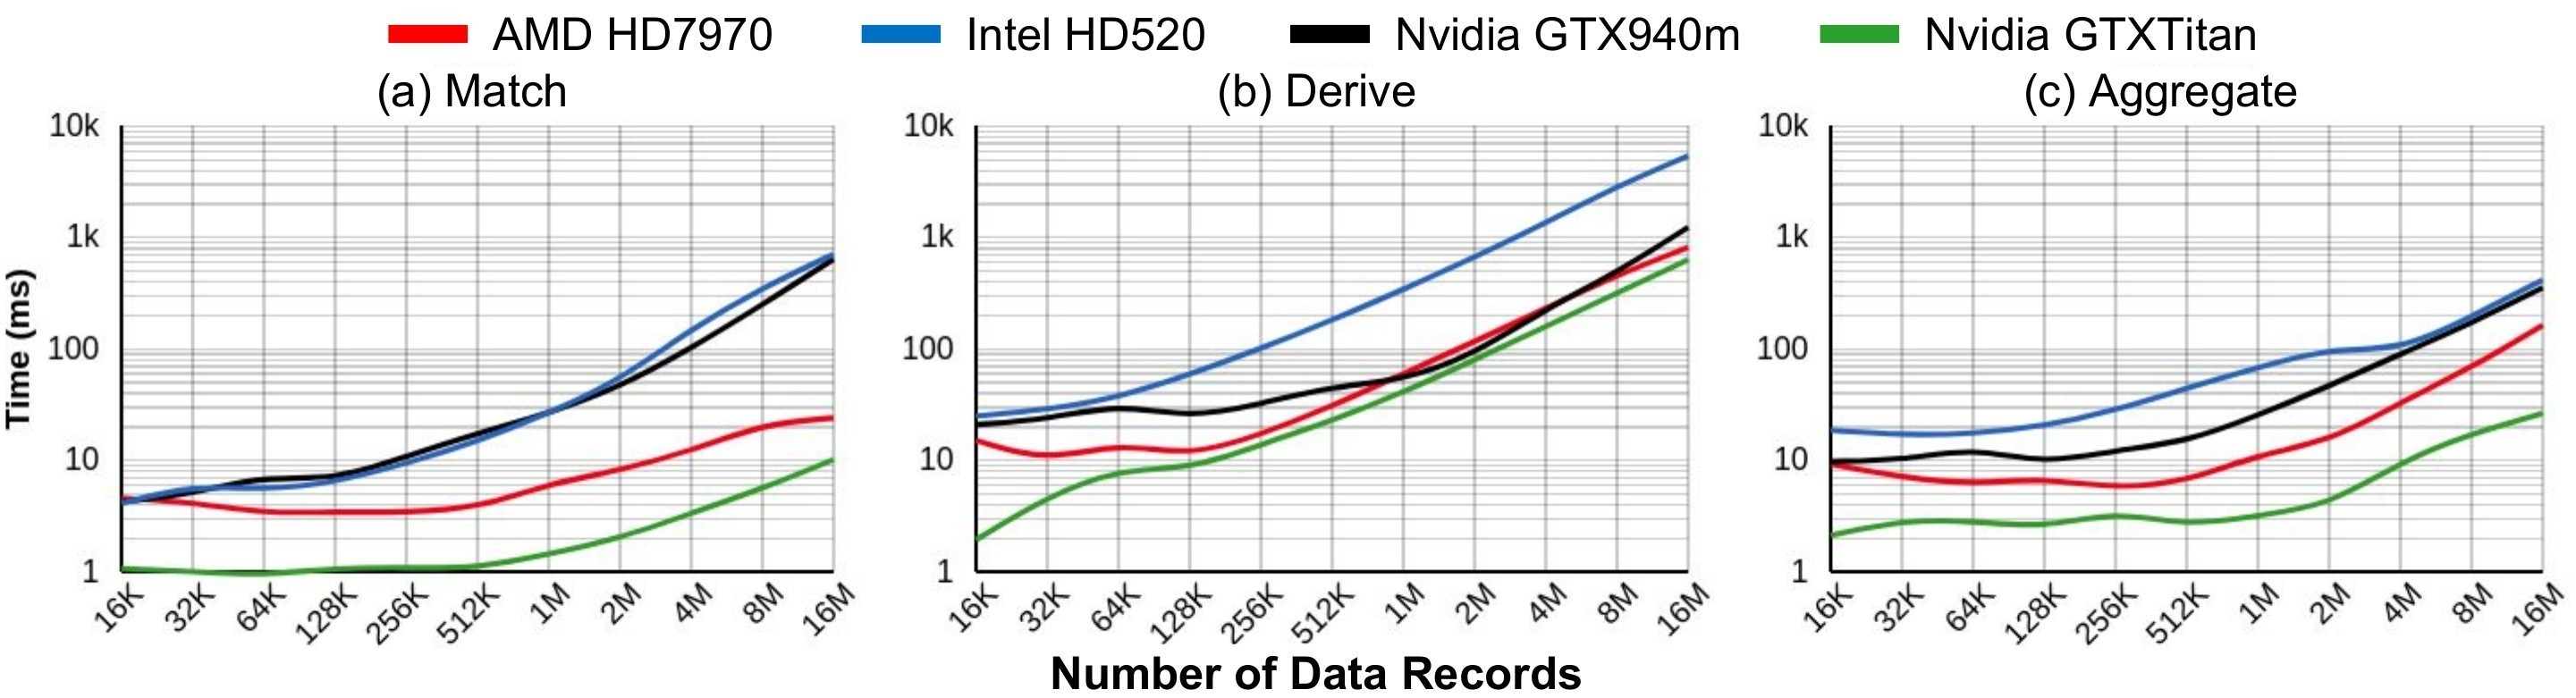
\includegraphics[width=\textwidth,keepaspectratio]{img/mineria/p4_14}
		%\label{img:mot2}
		\caption{Tiempo promedio de P4 y las demas librerías para procesar las tareas de \textit{Match}, \textit{Derive} y \textit{Aggregate}. Fuente: \cite{li2018p4}}
	\end{figure}
\end{frame}
%-------------------------------------------------------
%-------------------------------------------------------

%-------------------------------------------------------
%-------------------------------------------------------
\begin{frame}{Benchmark}{Desempeño en la transformación de datos}
	\begin{figure}[]
		\centering
		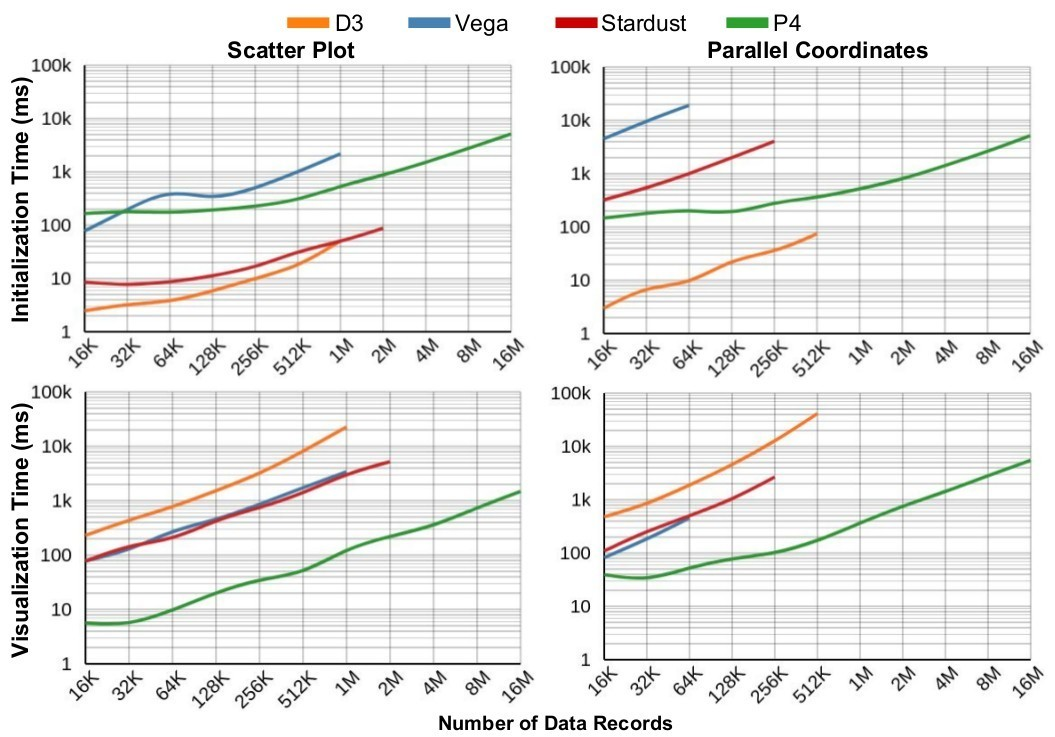
\includegraphics[width=0.8\textwidth,keepaspectratio]{img/mineria/p4_15}
		%\label{img:mot2}
		\caption{Comparación del tiempo promedio de inicialización y tiempo de visualización (tiempo por fotograma) con las demás librerías. Fuente: \cite{li2018p4}}
	\end{figure}
\end{frame}
%-------------------------------------------------------
%-------------------------------------------------------

%-------------------------------------------------------
%-------------------------------------------------------
\begin{frame}{Benchmark}{Desempeño en la transformación de datos}
	\begin{figure}[]
		\centering
		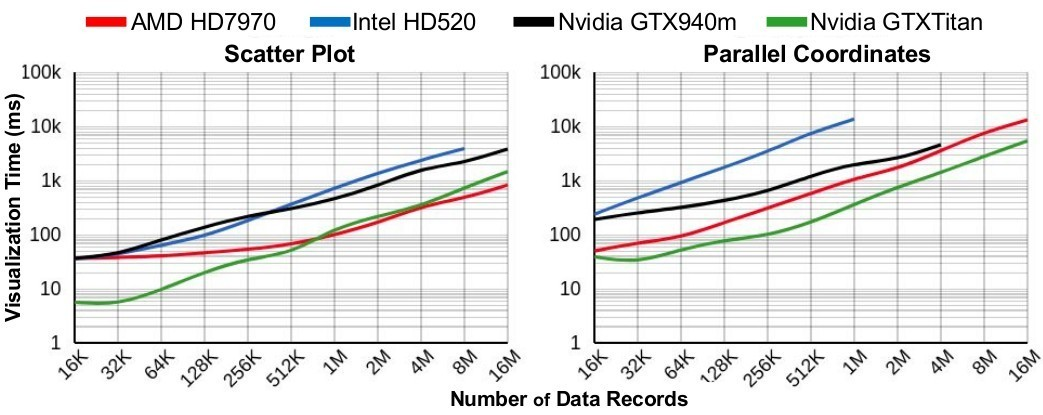
\includegraphics[width=0.9\textwidth,keepaspectratio]{img/mineria/p4_16}
		%\label{img:mot2}
		\caption{Comparación del tiempo promedio de inicialización y tiempo de visualización (tiempo por fotograma en varios GPUs. Fuente: \cite{li2018p4}}
	\end{figure}
\end{frame}
%-------------------------------------------------------
%-------------------------------------------------------


%%%%%%%%%%%%%%%%%%%%%%%%%%%%%%%%%%%%%%%%%%%%%%%%%%%%%%%%%%%%%%%%%%%%%%%%%%%%%%%%%%%%%%%%%%%%%%%%%%%%%%%%%%%%%%%%
%%%%%%%%%%%%%%%%%%%%%%%%%%%%%%%%%%%%%%%%%%%%%%%%%%%%%%%%%%%%%%%%%%%%%%%%%%%%%%%%%%%%%%%%%%%%%%%%%%%%%%%%%%%%%%%%
\section{Conclusiones}
%%%%%%%%%%%%%%%%%%%%%%%%%%%%%%%%%%%%%%%%%%%%%%%%%%%%%%%%%%%%%%%%%%%%%%%%%%%%%%%%%%%%%%%%%%%%%%%%%%%%%%%%%%%%%%%%
%%%%%%%%%%%%%%%%%%%%%%%%%%%%%%%%%%%%%%%%%%%%%%%%%%%%%%%%%%%%%%%%%%%%%%%%%%%%%%%%%%%%%%%%%%%%%%%%%%%%%%%%%%%%%%%%

%-------------------------------------------------------
%-------------------------------------------------------
\begin{frame}{Conclusiones}{}
	\begin{itemize}
	    \item Mientras que la mayoría de herramientas se enfocan en la expresividad, P4 combina el procesamiento con GPU y gramáticas declarativas.
	    \item P4 es mas rapido que otras herramientas de  transformación y visualización de datos.
	    \item El desempeño de P4 depende fuertemente de la capacidad del GPU.
	    \item Comparado con P4, $D^3$ tiene mejor expresividad para la visualización de datos.
	\end{itemize}
\end{frame}
%-------------------------------------------------------
%-------------------------------------------------------










%-------------------------------------------------------
%-------------------------------------------------------
\begin{frame}[allowframebreaks]
\frametitle{References}
%\bibliographystyle{amsalpha}
\bibliographystyle{IEEEtran}
\bibliography{bibliography.bib}
\end{frame}
%-------------------------------------------------------
%-------------------------------------------------------


%-------------------------------------------------------
%-------------------------------------------------------
\if\mycmd1 % MY THEME
	\begin{frame}[plain,noframenumbering]
		%\finalpage{Thank you}
		\begin{figure}[]
			\centering
			
\includegraphics[width=\textwidth,height=0.7\textheight,keepaspectratio]{img/question.png}
			%\label{img:mot2}
			%\caption{Image example in 2 gray levels.}
		\end{figure}
	\end{frame}
	
\else % CS THEME
\begin{frame}{Questions?}
	\begin{figure}[]
		\centering
		
\includegraphics[width=\textwidth,height=0.7\textheight,keepaspectratio]{img/question.png}
		%\label{img:mot2}
		%\caption{Image example in 2 gray levels.}
	\end{figure}
	
\end{frame}
\fi
%-------------------------------------------------------
%-------------------------------------------------------
	
	
\end{document}